
\chapter{Consequences for the Belle~II Experiment}
\label{chap:Conseqences}

	Simulations of the expected neutron flux in full Belle~II running at the design luminosity of 8$\times10^{35}$ cm$^{-2}$s$^{-1}$ with residual gas pressure of 10~nTorr were calculated using SAD to simulate collider conditions and GEANT4 to simulate the detector. Table \ref{tab:neutronFluxTable} shows the highest neutron flux expected in each subdetector, as predicted by SAD and GEANT4. Figures showing the expected neutron flux in each subdetector can be found in Figs~\ref{fig:VXDFlux}-\ref{fig:EKLMForFlux}.


\begin{table}[ht]
	\centering
	\begin{tabular}{ lSSSS }	
	&	{Maximum}	&		&	{Maximum}	&		\\	
	&	{Neutron Flux}	&		&	{Neutron Flux}	&		\\	
	&	{No Re-weighting}	&	{Tolerance}	&	 {After Re-weighting}	&		\\	
Subdetector	&	{($\times10^{9}$cm$^{-2}$yr$^{-1}$)} 	&	{($\times10^{9}$cm$^{-2}$yr$^{-1}$)} 	&	{($\times10^{9}$cm$^{-2}$yr$^{-1}$)}	&	{\% increase}	\\	\hline \hline
PXD	&	92	&		&	106	&	15.7	\\	
SVD	&	373	&		&	421	&	12.9	\\	
CDC	&	57	&	100	&	70	&	23.0	\\	
ARICH	&	104	&	100	&	115	&	9.8	\\	
TOP – Bars	&	46	&	50	&	56	&	19.7	\\	
TOP – Electronics	&	16	&		&	21	&	28.5	\\	
ECL - Forward	&	23	&	100	&	24	&	3.8	\\	
ECL - Barrel	&	5	&	100	&	6	&	26.2	\\	
ECL - Backward	&	14	&	100	&	19	&	36.0	\\	
BKLM	&	0.37	&		&	0.46	&	23.6	\\	
EKLM - Forward	&	1.88	&		&	2.26	&	20.0	\\	
EKLM - Backward	&	1.56	&		&	1.72	&	10.8	\\	\hline

	\end{tabular}
	\caption[Neutron flux as predicted by SAD and GEANT4]{Neutron flux as predicted by SAD and GEANT4.}
	\label{tab:neutronFluxTable}
\end{table}




Using the parameters $(D/S)_{\mathrm{gas}}$ and $(D/S)_{\mathrm{T}}$ described in \S~\ref{sec:TousExp}, the beam-gas and Touschek components of these simulations can be re-weighted to improve the prediction of the neutron flux. The Belle~II subdetector most affected by the re-weighting of the beam-gas and Touschek simulation is the backward part of the ECL. Fortunately, the predicted neutron flux, though increased, is still well below the tolerance. There are four different background components: Touschek, beam-gas, and two radiative Bhabha components. Only the Touschek and beam-gas components can be re-weighted at this time. The TOP and ARICH, while showing smaller increases, are both slightly outside their tolerances, as shown in Fig \ref{fig:increasePlot}. The average increase for all subdetectors is $\sim$20\%, which is a significant increase. Further thought must be given to mitigating this higher than expected neutron flux, such as additional neutron shielding. It might also be necessary to replace components as they become too irradiated.


Since there were no collisions in Phase~I, there is no information on the radiative Bhabha backgrounds, and they can not be re-weighted at this time. The cross section for this process is well understood, and does not require simulation of the collider with SAD. It does, however, require GEANT4 simulation. This will assist in determining whether SAD or GEANT4 is the source of the discrepancy between data and simulation.



%Although the cross section for this process is well understood, which reduces the uncertainty from this background, the source of neutron production induced by this process still relies on GEANT4 simulation of Belle~II. 


\begin{figure}[htb]
	\centerfloat
		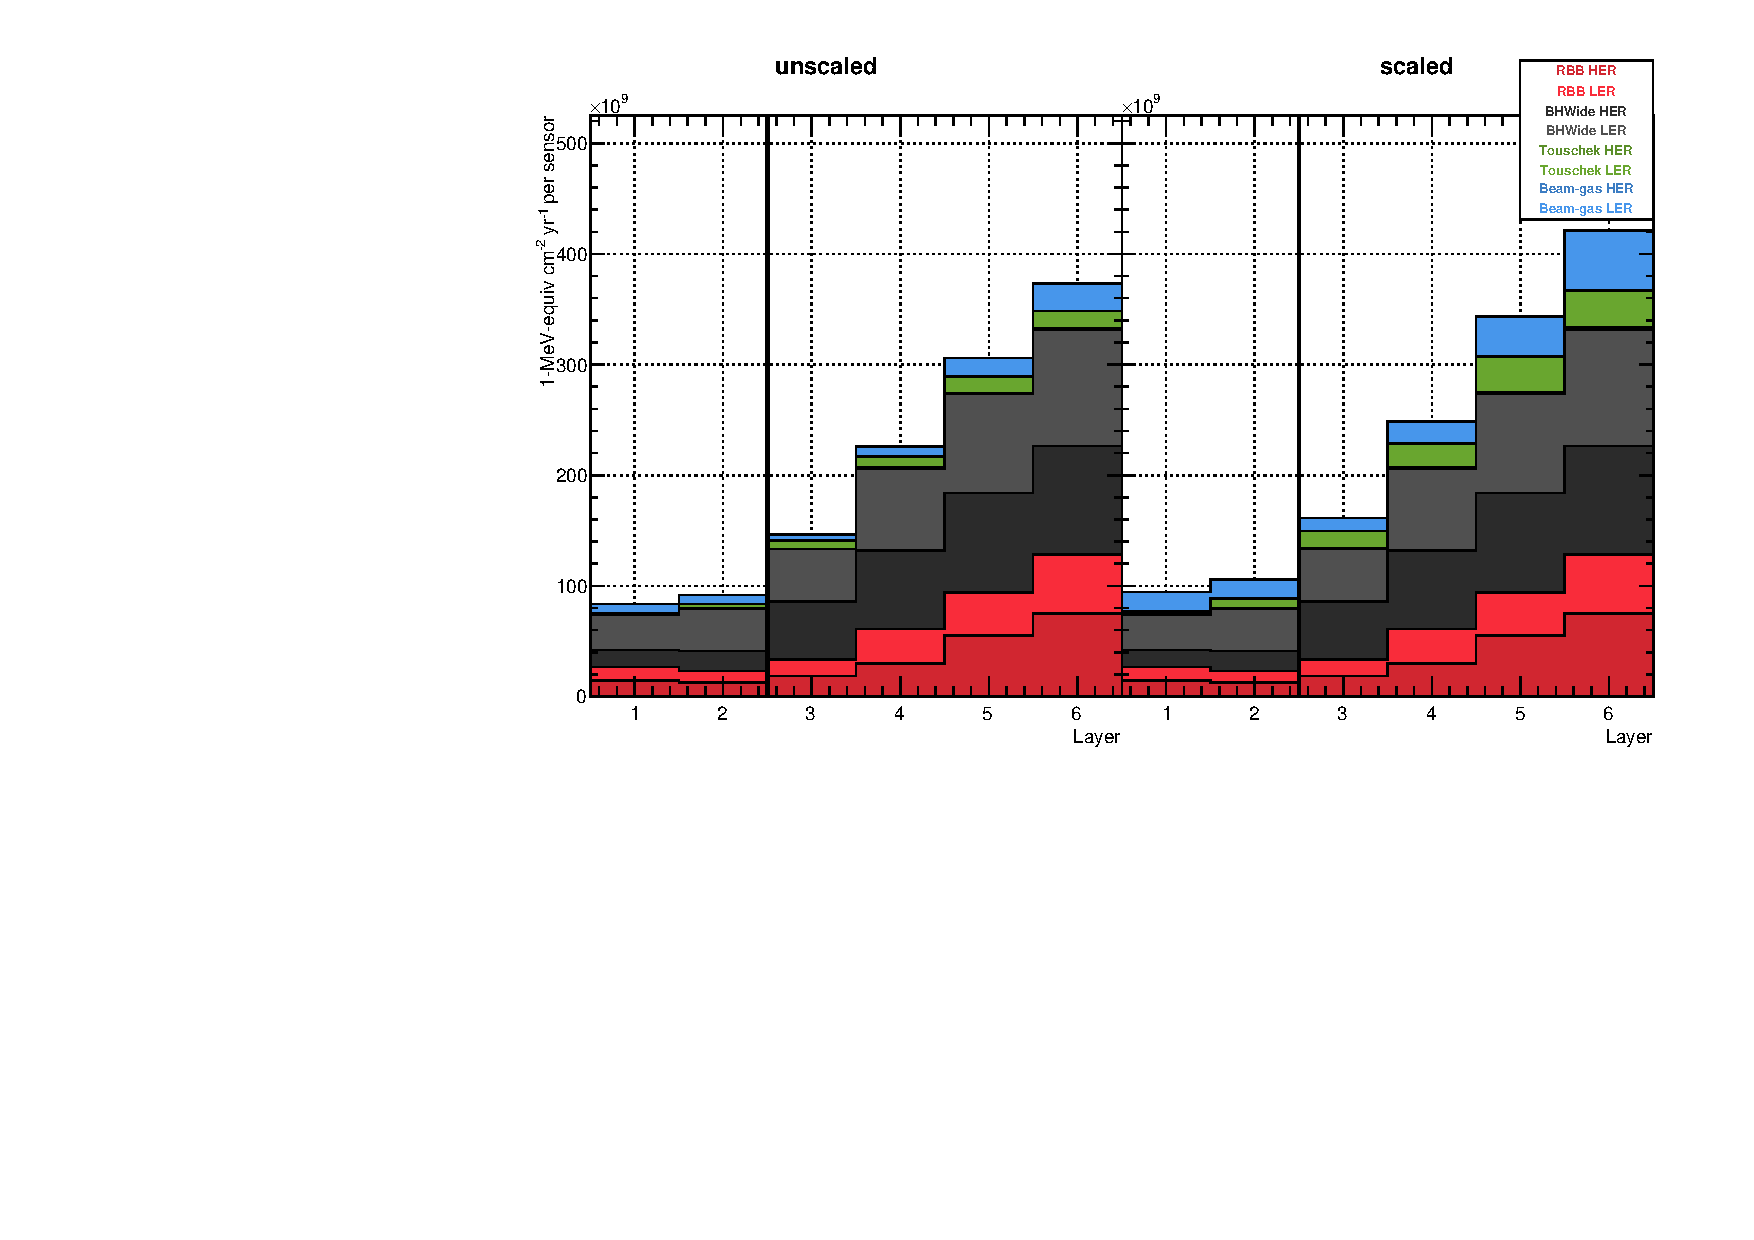
\includegraphics[width=\textwidth]{images/hVXDFlux}
	\caption[Neutron flux in VXD]{Neutron flux in VXD. Layers 1 \& 2 are the PXD and 3-6 are the SVD.}	
	\label{fig:VXDFlux}
\end{figure}

\begin{figure}[htb]
	\centerfloat
		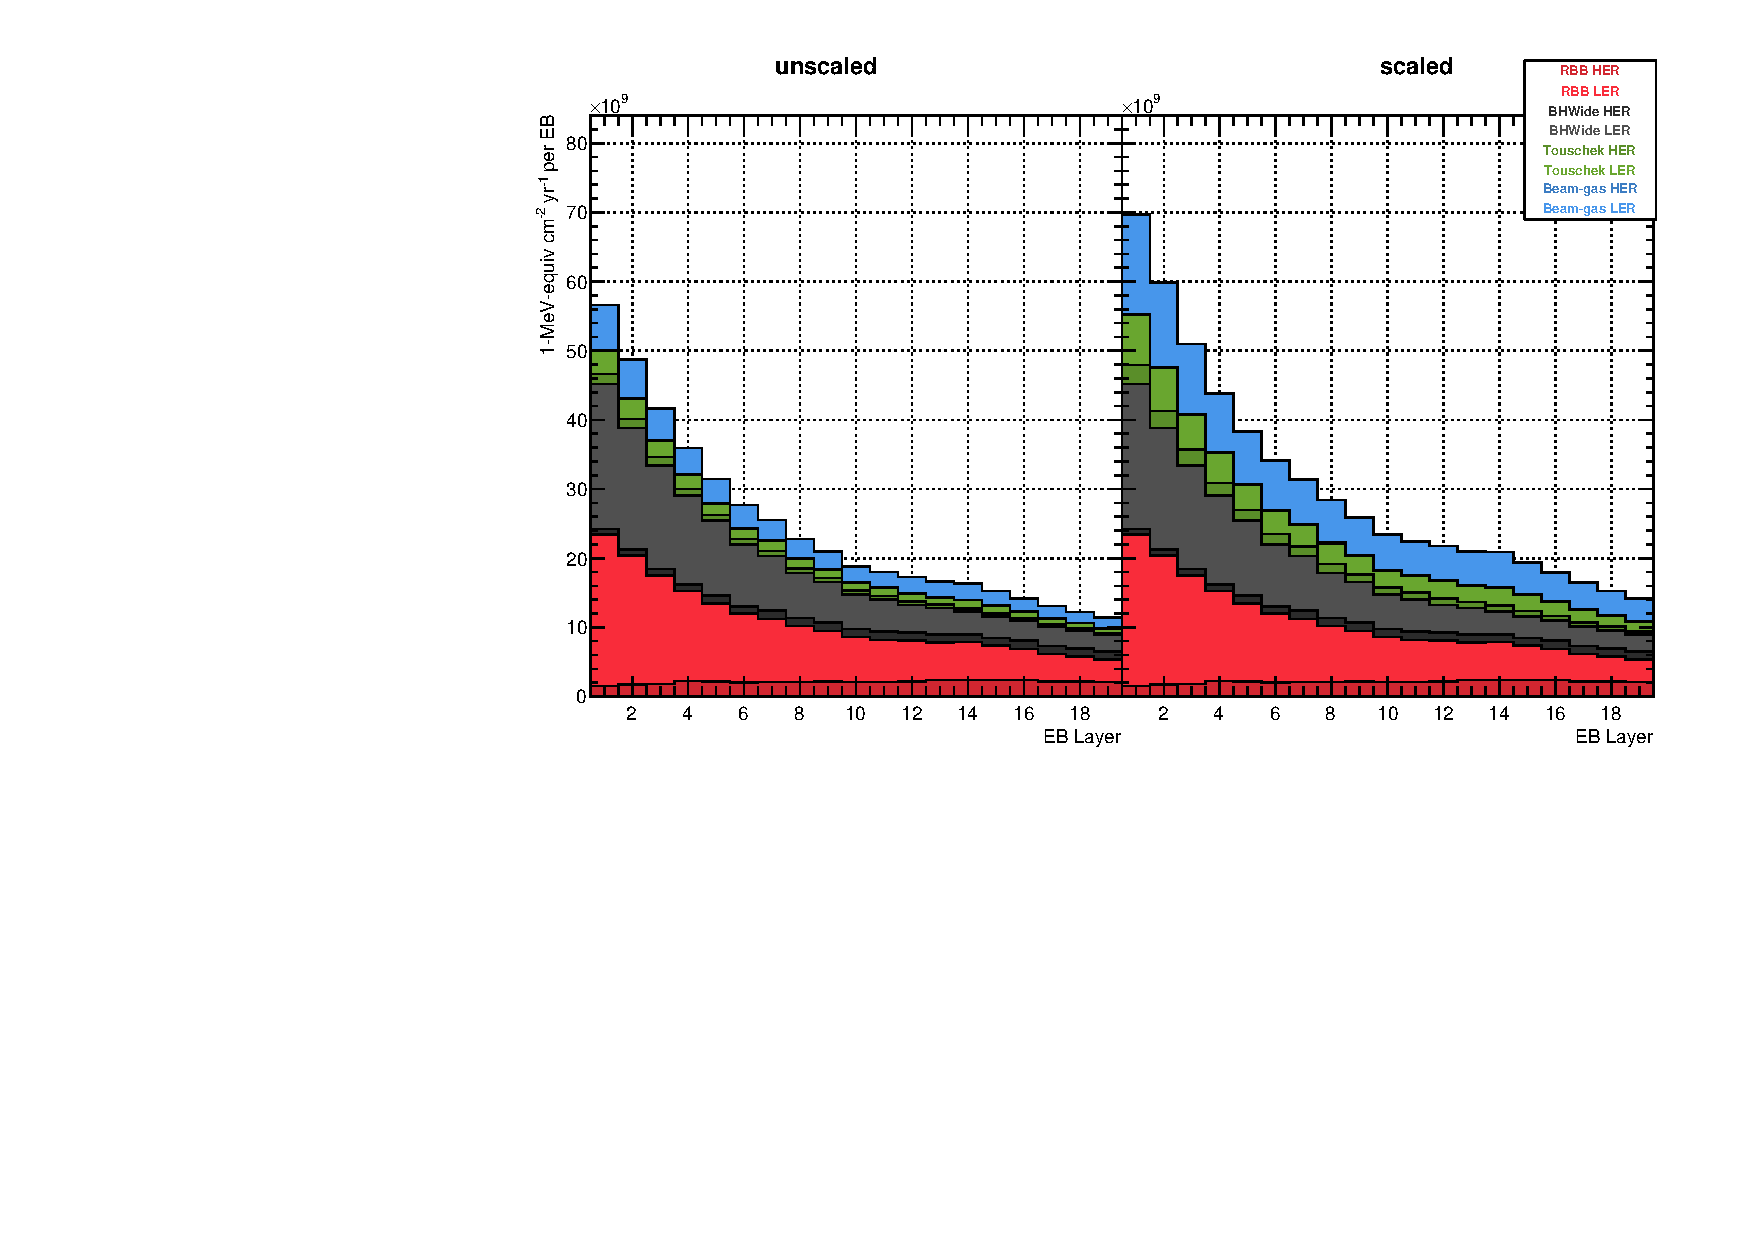
\includegraphics[width=\textwidth]{images/hCDCFlux}
	\caption[Neutron flux in CDC electronics]{Neutron flux in CDC electronics. Layer 1 is the innermost layer. Larger layer numbers correspond to higher radii.}	
	\label{fig:CDCFlux}
\end{figure}

\begin{figure}[htb]
	\centerfloat
		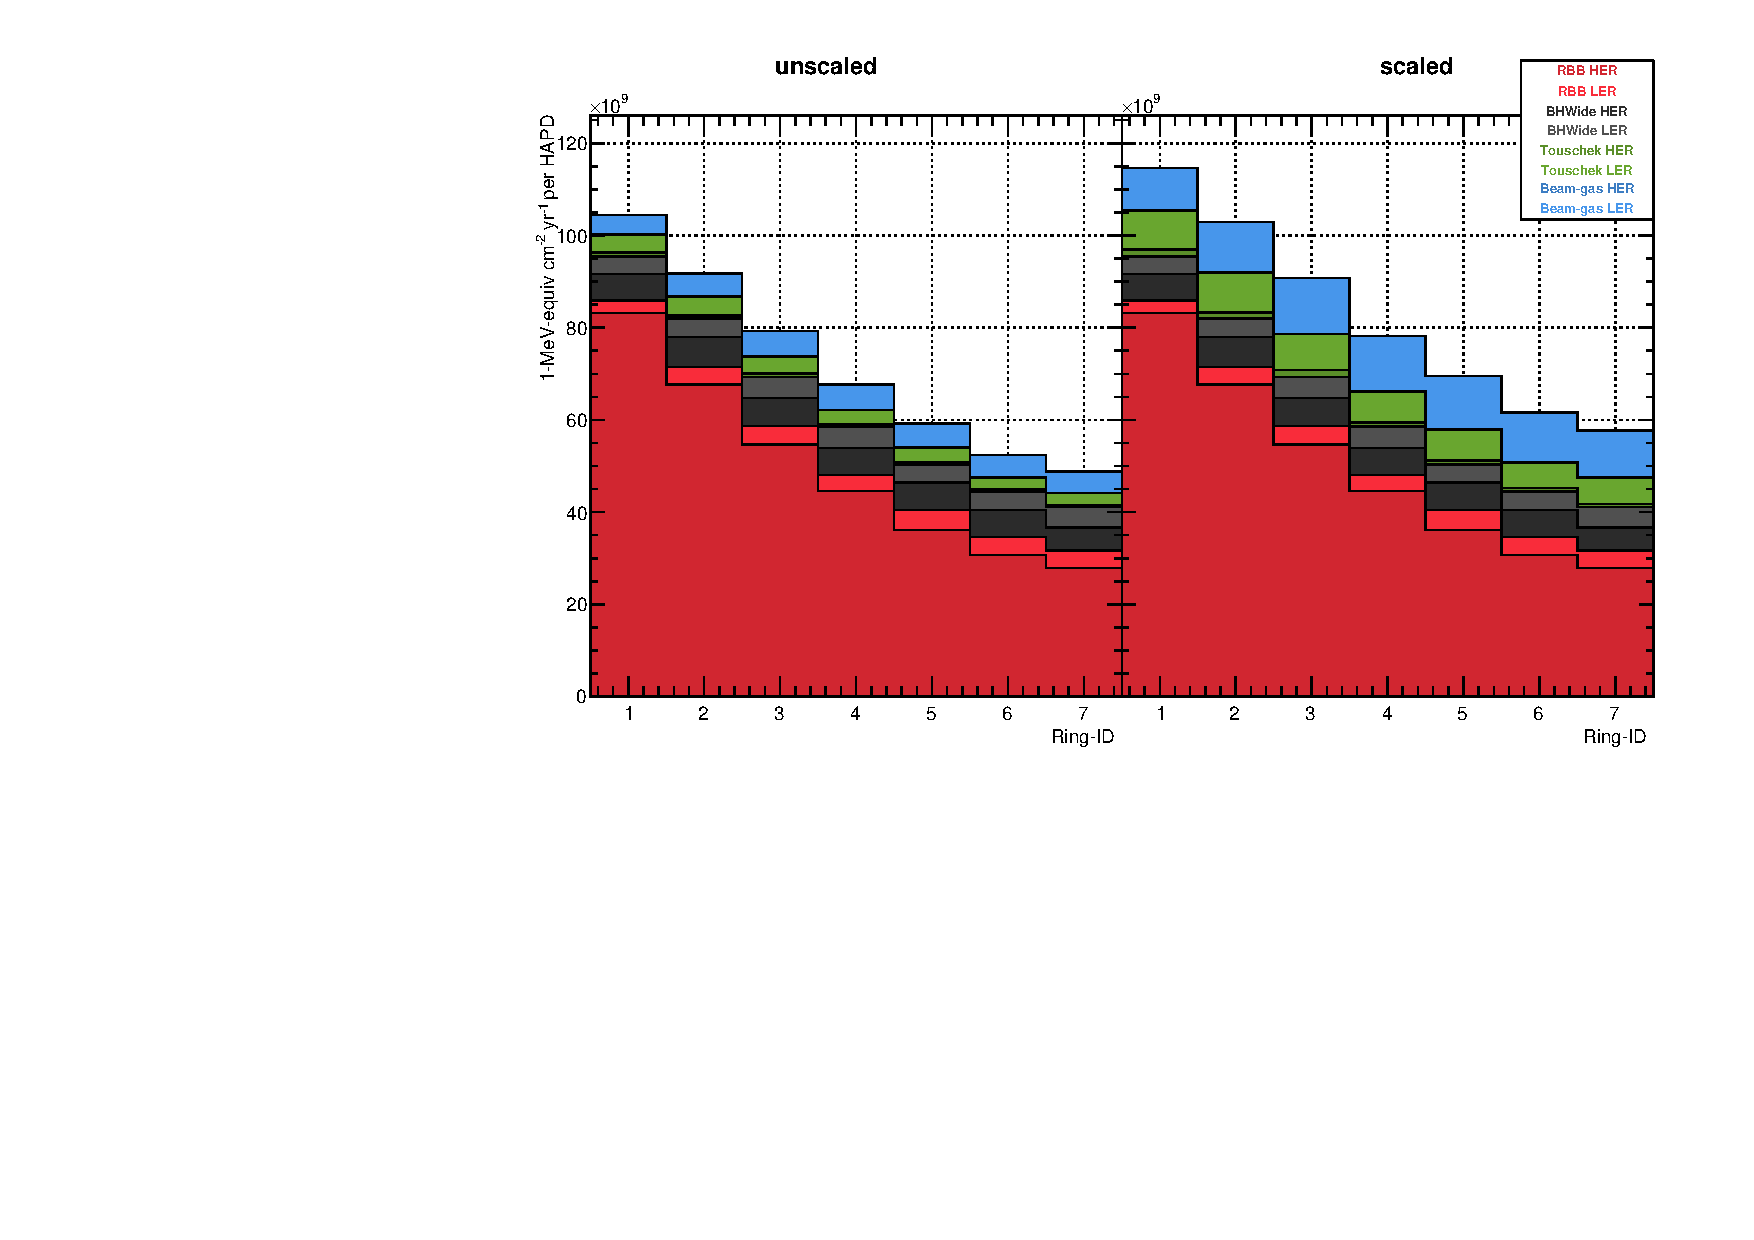
\includegraphics[width=\textwidth]{images/hARICHFlux}
	\caption[Neutron flux in ARICH rings]{Neutron flux in ARICH Rings. Ring-ID of 1 is the innermost ring. Ring-ID increases with radius.}	
	\label{fig:ARICHFlux}
\end{figure}

\begin{figure}[htb]
	\centerfloat
		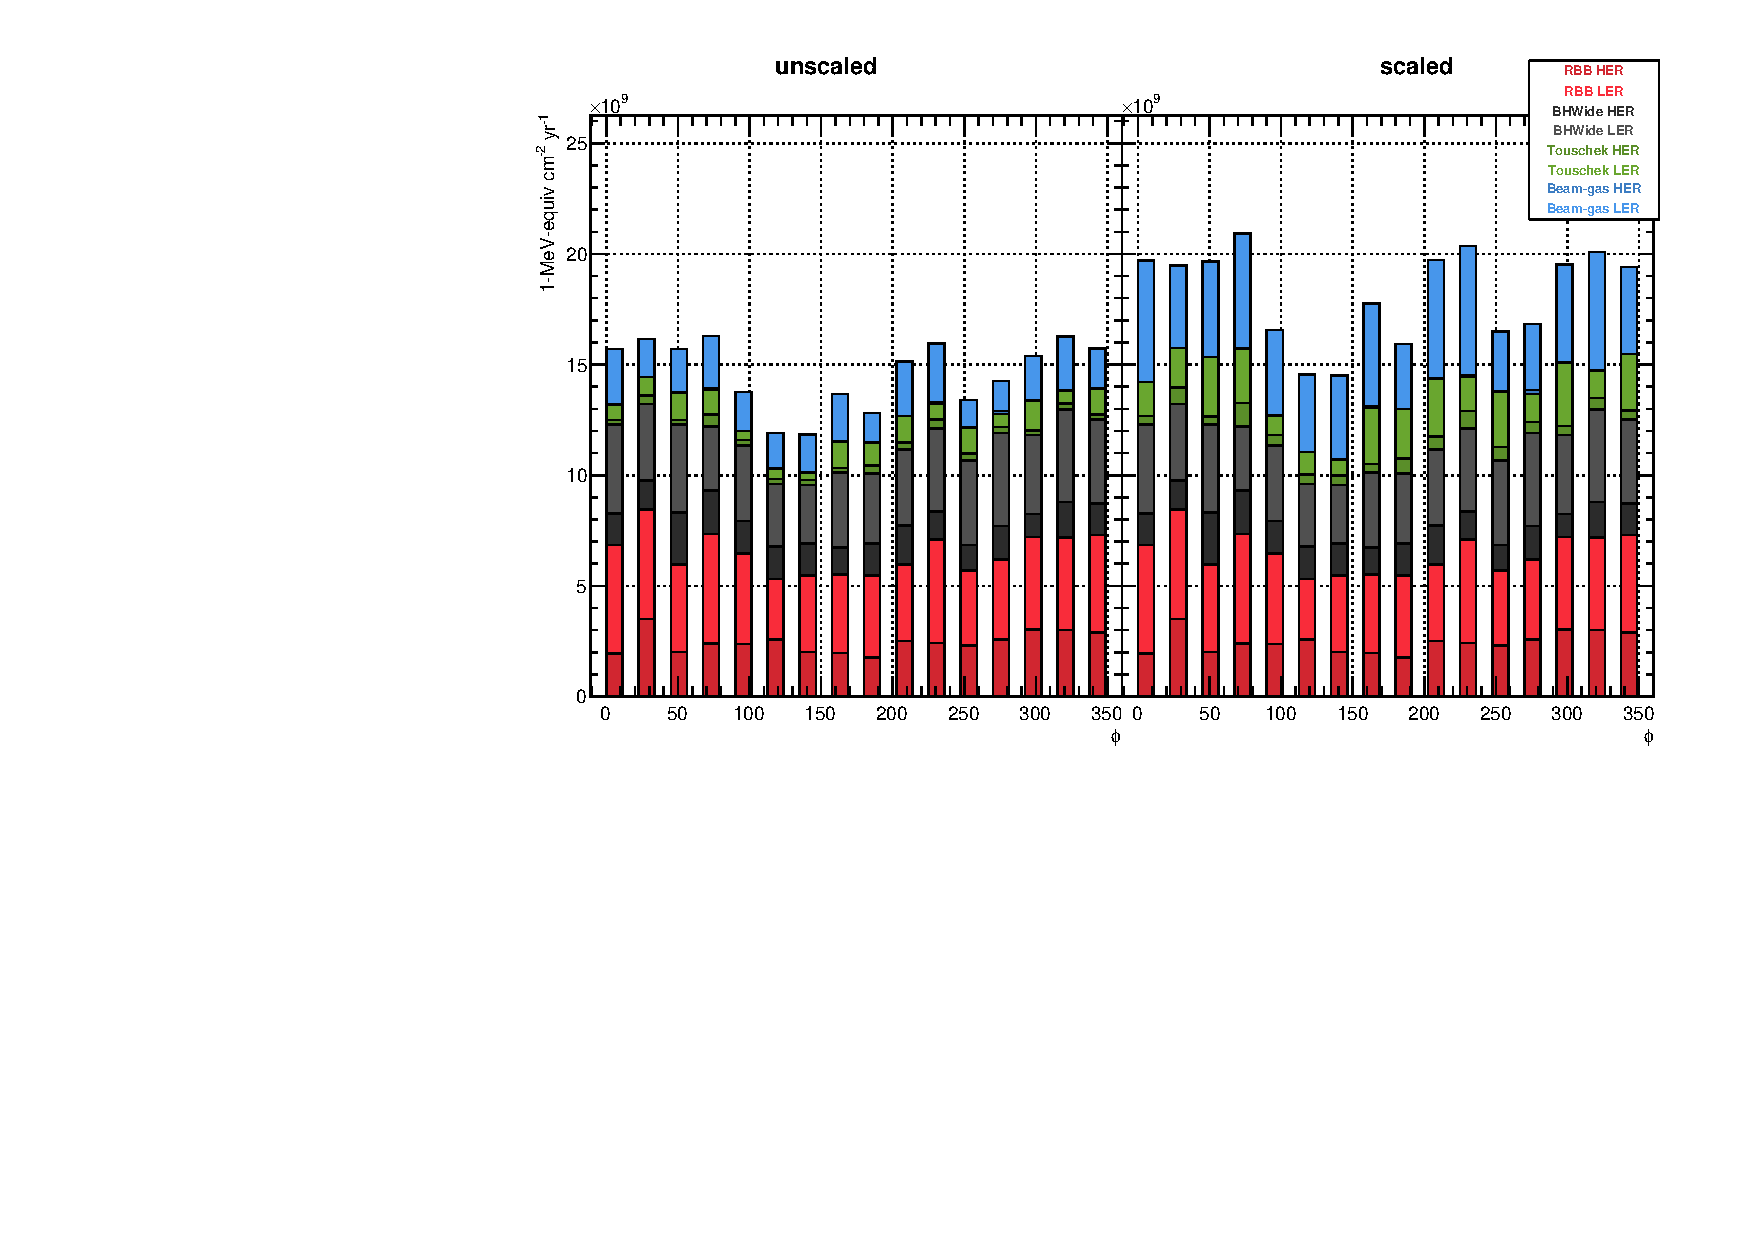
\includegraphics[width=\textwidth]{images/hTOPFlux}
	\caption[Neutron flux in TOP electronics]{Neutron flux in TOP electronics.}	
	\label{fig:TOPFlux}
\end{figure}

\begin{figure}[htb]
	\centerfloat
		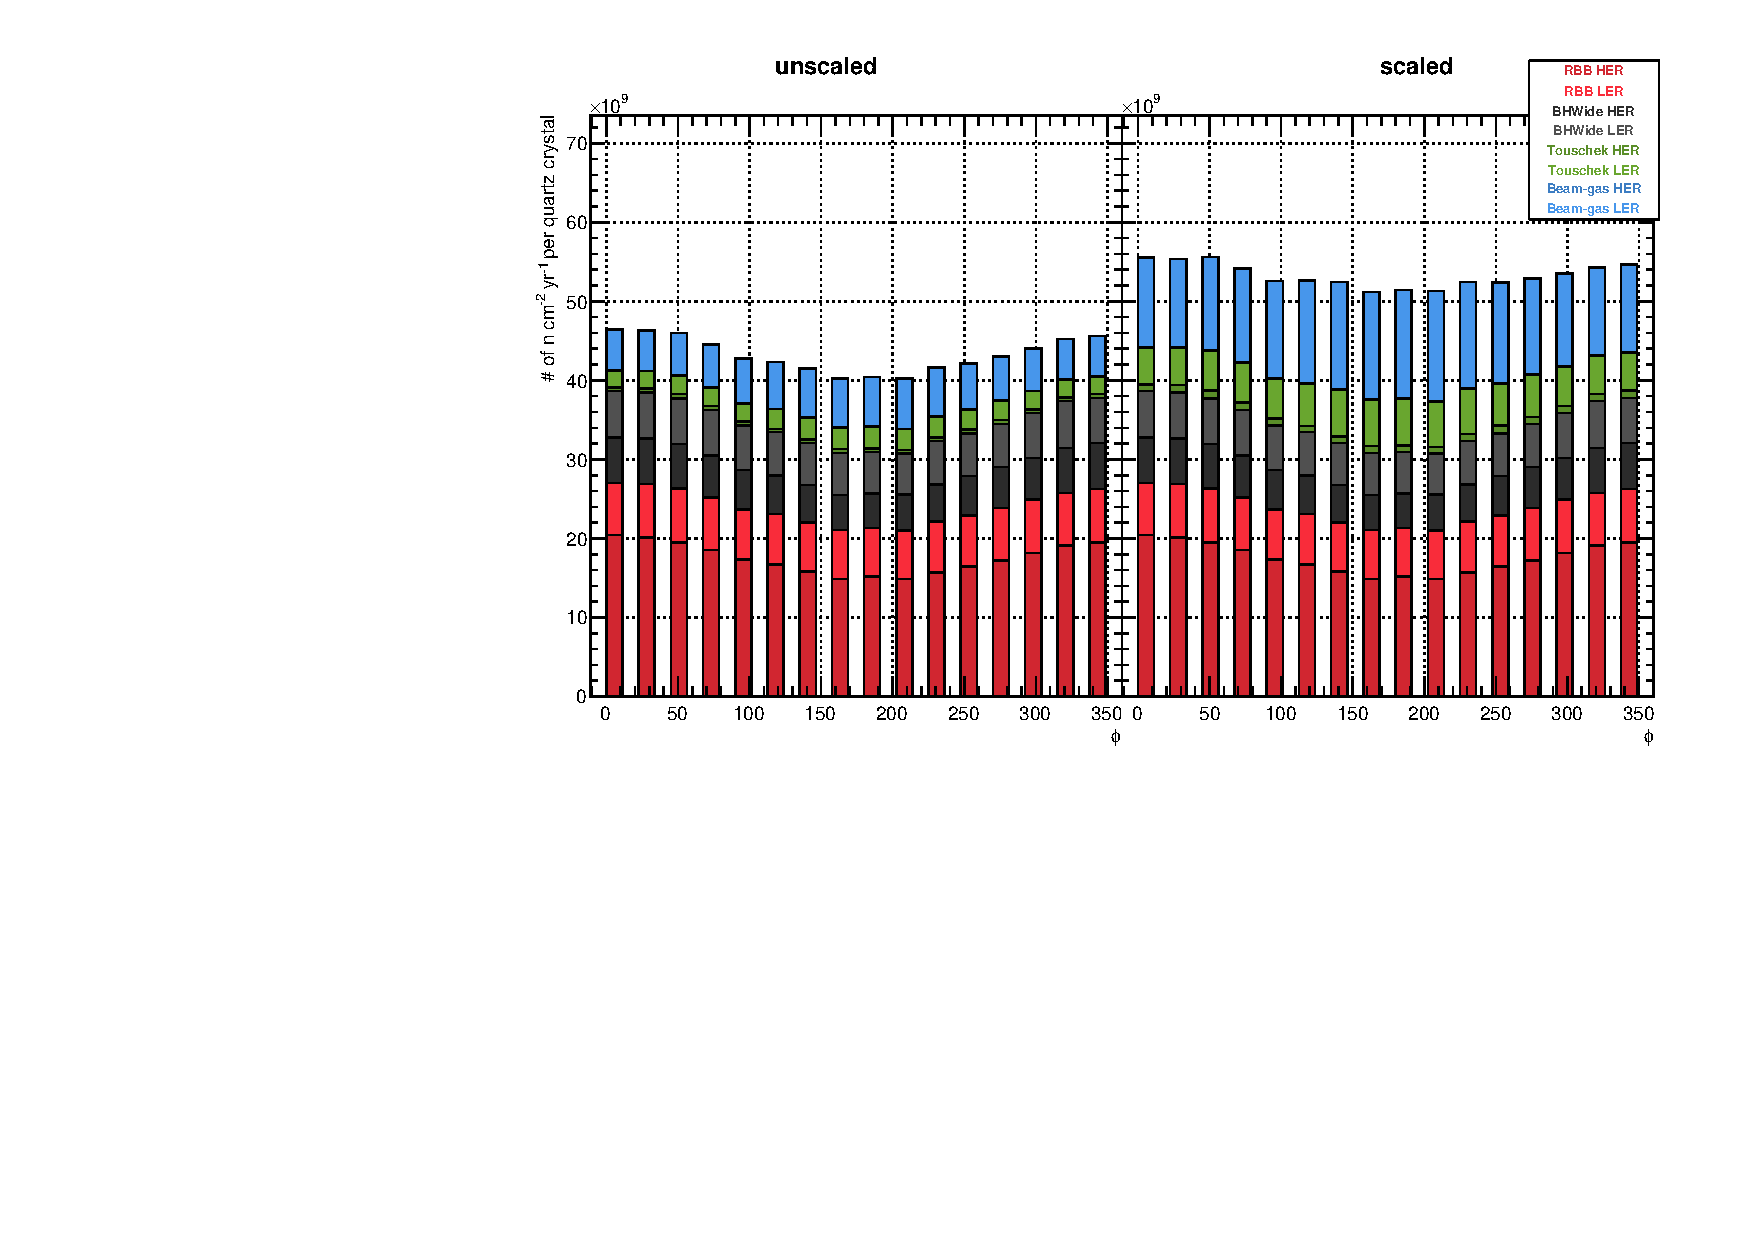
\includegraphics[width=\textwidth]{images/hTOPFluxBar}
	\caption[Neutron flux in TOP quartz bars]{Neutron flux in TOP quartz bars.}	
	\label{fig:TOPBARFlux}
\end{figure}

\begin{figure}[htb]
	\centerfloat
		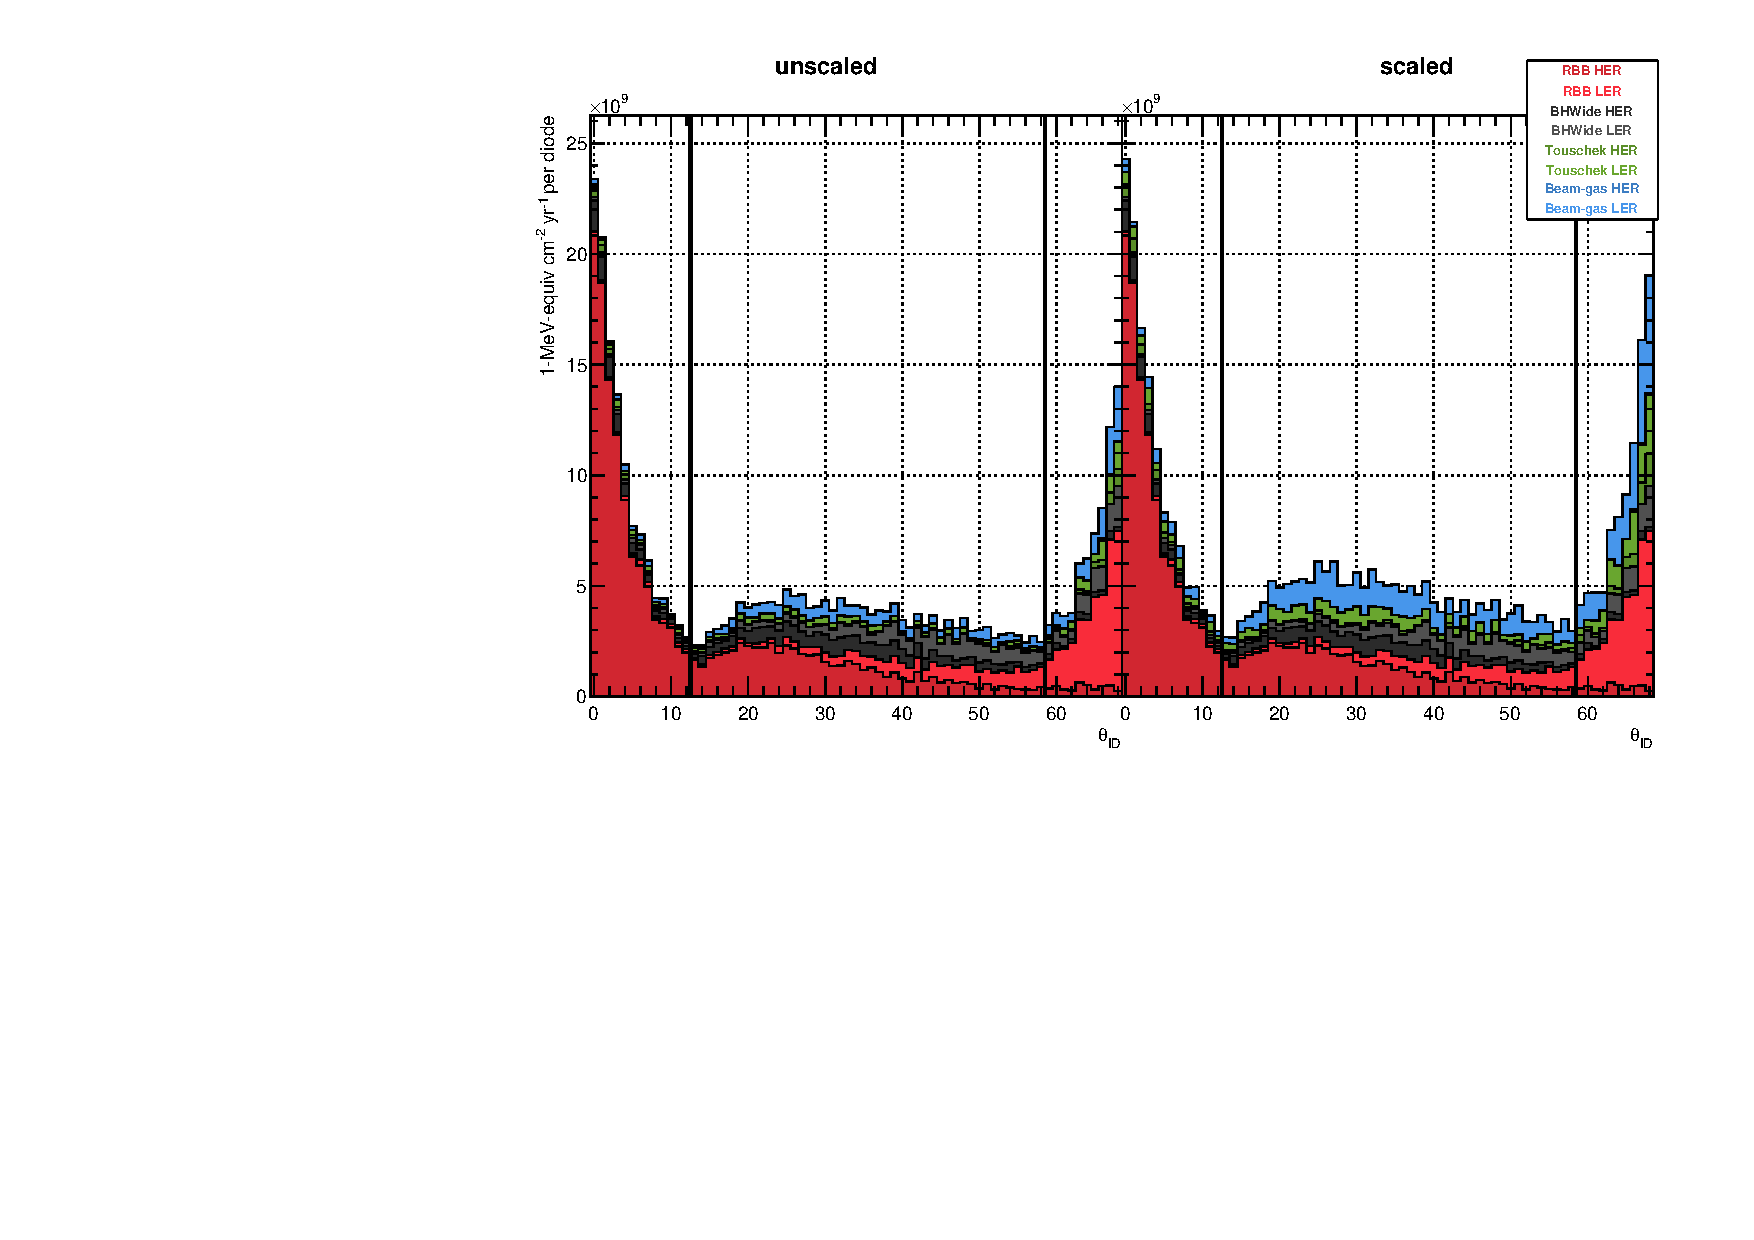
\includegraphics[width=\textwidth]{images/hECLFluxTID}
	\caption[Neutron flux in ECL diodes]{Neutron flux in ECL diodes. Explanation of $\theta_{ID}$ can be found in Appendix \ref{chap:THID}.}	
	\label{fig:ECLFlux}
\end{figure}

\begin{figure}[htb]
	\centerfloat
		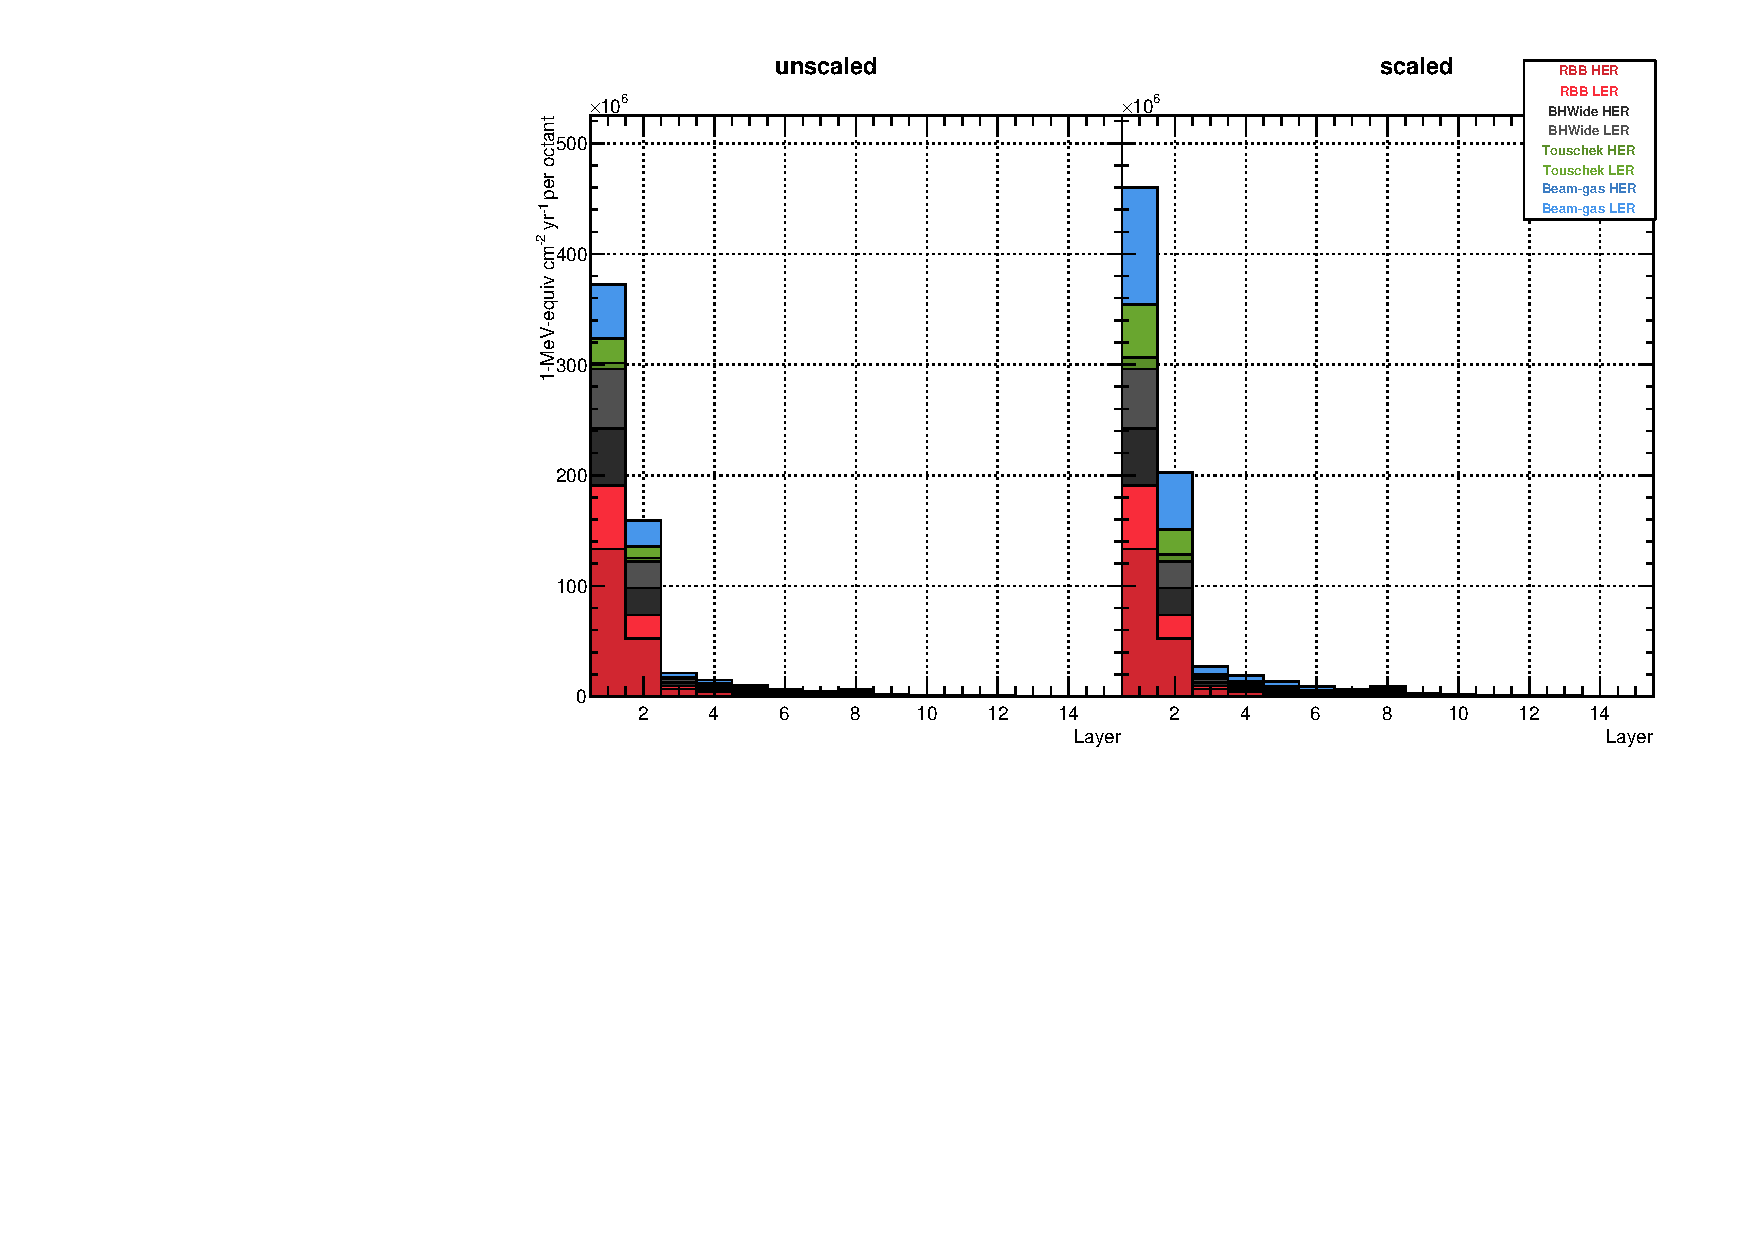
\includegraphics[width=\textwidth]{images/hBKLMFlux}
	\caption[Neutron flux in BKLM]{Neutron flux in BKLM. Layer 1 is the innermost layer. Layer increases with radius.}	
	\label{fig:BKLMFlux}
\end{figure}

\begin{figure}[htb]
	\centerfloat
		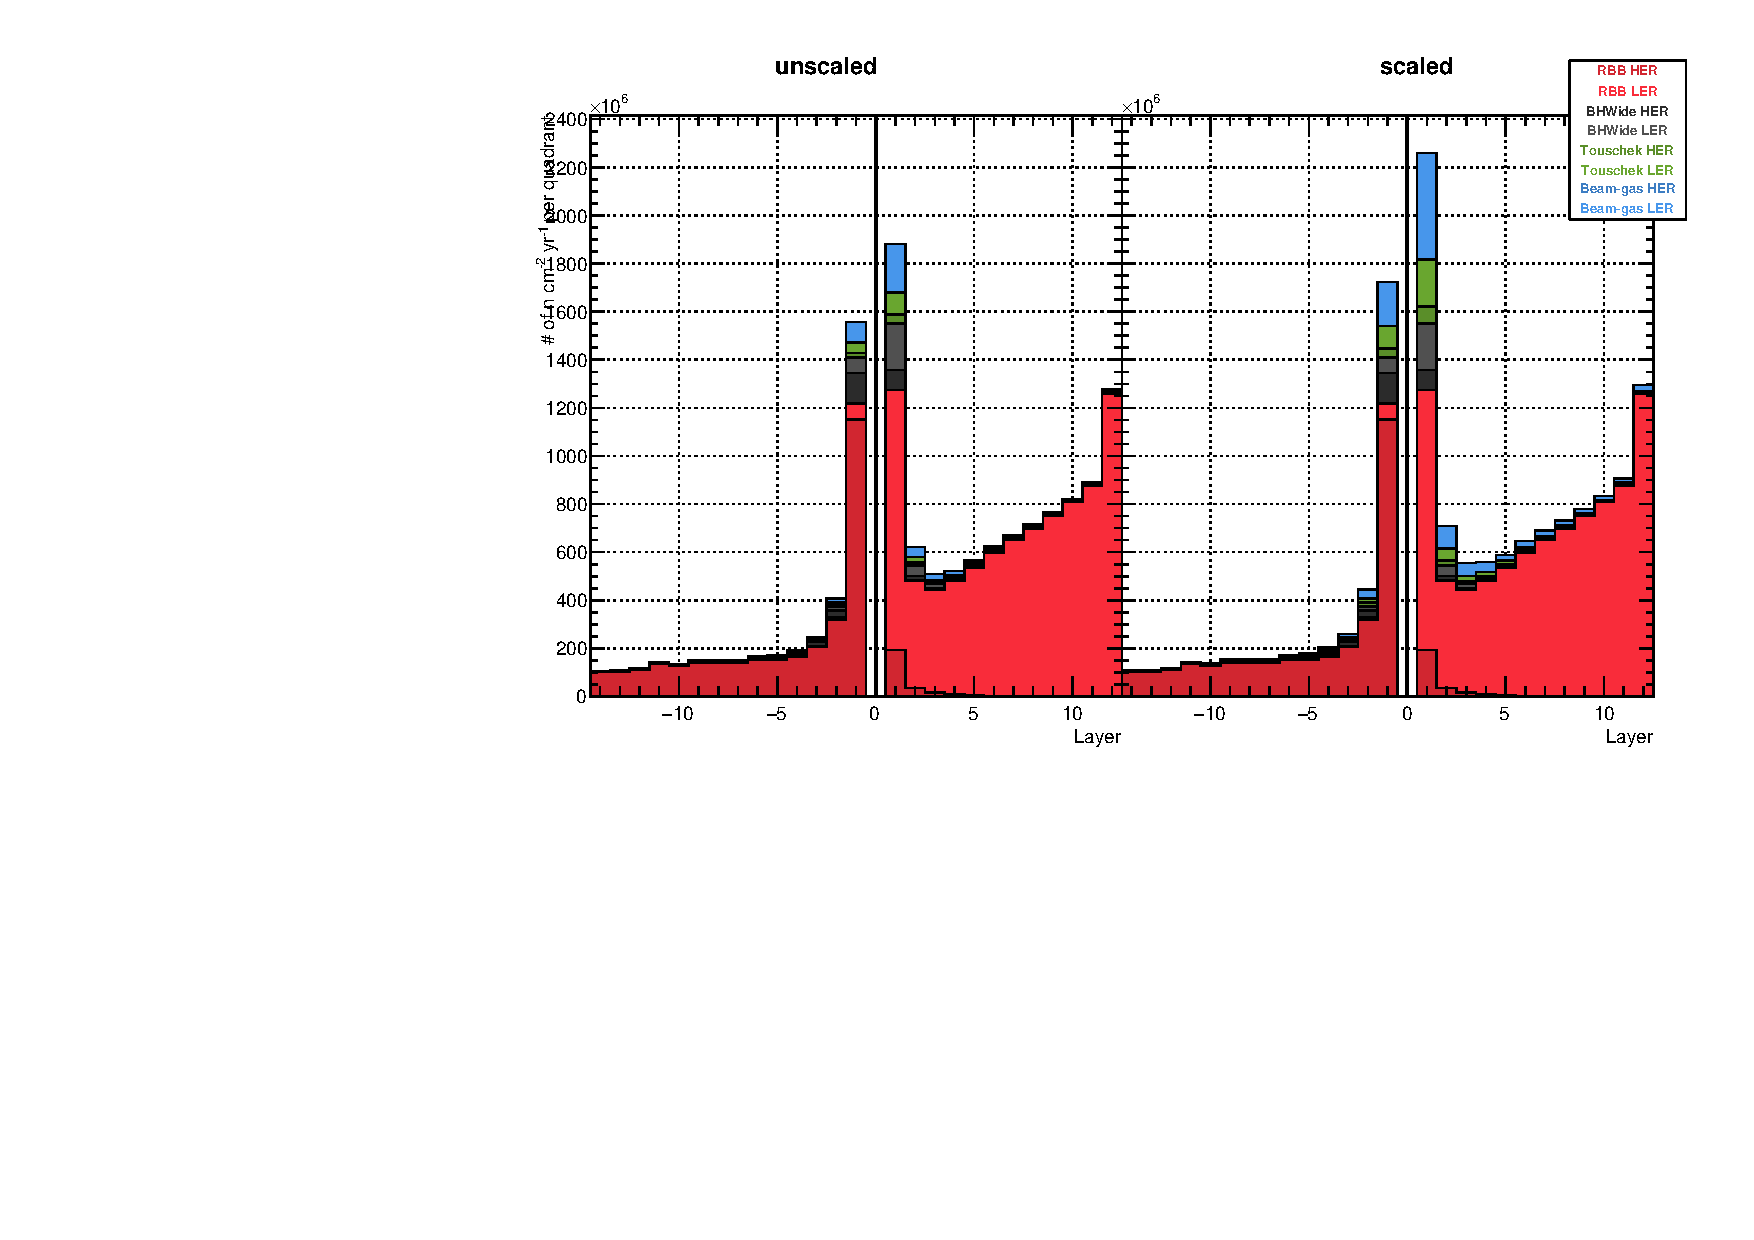
\includegraphics[width=\textwidth]{images/hEKLMFlux}
	\caption[Neutron flux in EKLM]{Neutron flux in EKLM. Negative layers are backward end-cap, positive layers are forward end-cap. Layers 1 and -1 are closest to IR.}	
	\label{fig:EKLMForFlux}
\end{figure}



\begin{figure}
	\centerfloat
		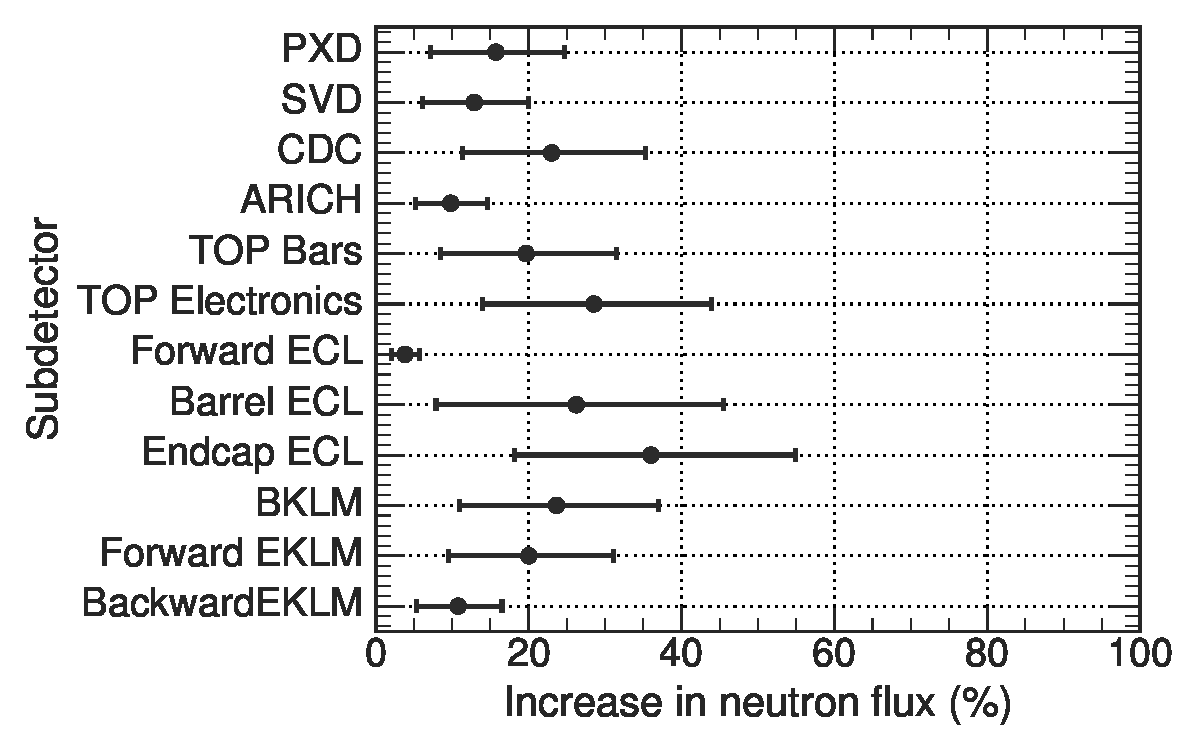
\includegraphics[width=\textwidth]{images/IncreasePlot}
	\caption[Increase in background flux in each detector]{Increase in background flux in each detector.}
	\label{fig:increasePlot}
\end{figure}




























